\documentclass[11pt]{beamer}
\usetheme{Pittsburgh}
\usepackage[utf8]{inputenc}
\usepackage{amsmath}
\usepackage{amsfonts}
\usepackage{pifont}
\newcommand{\cmark}{\ding{51}}%
\newcommand{\xmark}{\ding{55}}%
\usepackage{amssymb}
\usepackage{todonotes}
\usepackage{ragged2e} 
\usepackage{comment}
\usepackage{enumitem}
\usepackage{tikz}
\usepackage{pgfgantt} 
\usepackage{listings}
\setcounter{tocdepth}{2}% Allow only section(1) and subsection(2), no subsubsection (3), in ToC

\setlist[itemize]{label=\textcolor{blue}{\textbullet}}
\newcommand{\xitem}{\item[\textcolor{red}{\xmark}]}
\newcommand{\citem}{\item[\textcolor{olive}{\cmark}]}

\author{Benjamin Rüth}
\title{Bokeh: A Python Plotting Library for the Web Browser}
\subtitle{Presentation at BGCE Research Day, TUM}
%\setbeamercovered{transparent} 
\setbeamertemplate{navigation symbols}{}%remove navigation symbols
%\logo{} 
%\institute{} 
\date{\today} 
%\subject{} 

\AtBeginSection[]
{
  \begin{frame}
    \frametitle{Table of Contents}
    \tableofcontents[currentsection]
  \end{frame}
}

\begin{document}
\setbeamertemplate{caption}{\raggedright\insertcaption\par}

\begin{frame}
\titlepage
\end{frame}

\section{Why do we need web visualization?}
\begin{frame}
\frametitle{\insertsection}
\textbf{Phase Plane Pictures: Source, Sink, Saddle}\\
Gilbert Strang, MIT\footnote{\url{https://www.youtube.com/watch?v=VqXKa11IA6A}}
\begin{center}
\only<1>{
the task\\
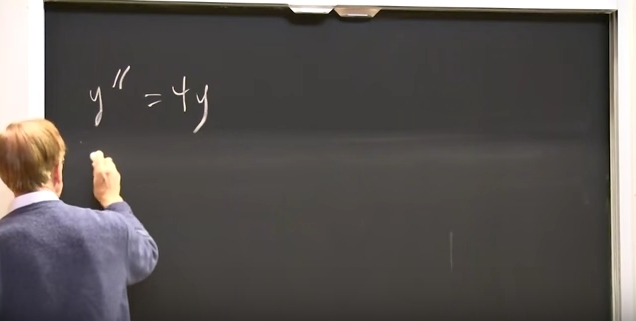
\includegraphics[width=.8\textwidth]{Pictures/Strang1.jpg}}
\only<2>{
3 minutes later\\
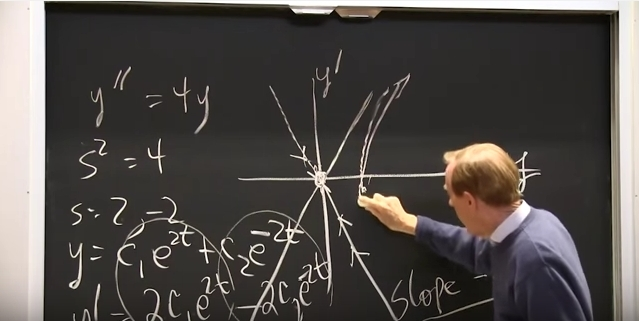
\includegraphics[width=.8\textwidth]{Pictures/Strang2.jpg}}
\only<3>{
another 2 minutes later\\
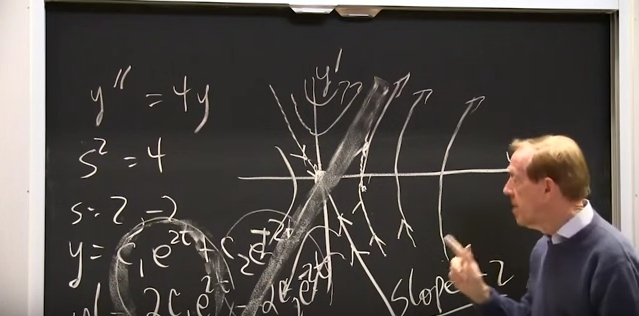
\includegraphics[width=.8\textwidth]{Pictures/Strang3.jpg}}
\end{center}
\end{frame}

\begin{frame}
\frametitle{\insertsection}
\begin{center}
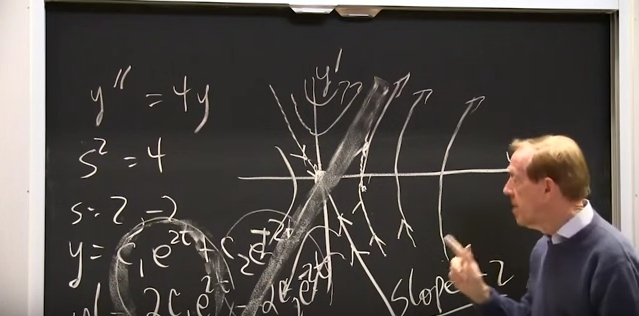
\includegraphics[width=.8\textwidth]{Pictures/Strang3.jpg}
\end{center}
\begin{block}{Problem with Videos and Lectures}
\begin{itemize}
\item Advisor needed
\item Time intensive
\item Not interactive (videos)
\item Not individual
\end{itemize}
\end{block}
\end{frame}

\section{Interactive Web Visualization}

\subsection{What do we want?}
\begin{frame}
\frametitle{\insertsubsection}
\begin{block}{Our goal}
\begin{itemize}
\item Visualization of math content
\item Easy-to-use, flexible tool
\item For use at home and in lectures
\end{itemize}
\end{block}
\pause
\begin{block}{User Constraints}
\begin{itemize}
\item No programming experience required
\item No special tools required
\end{itemize}
\end{block}
\pause
\begin{block}{Development Constraints}
\begin{itemize}
\item Easy to implement and understand
\item Support for scientific applications
\end{itemize}
\end{block}

\end{frame}

\subsection{Bokeh}
\begin{frame}
\frametitle{\insertsubsection}
\begin{figure}
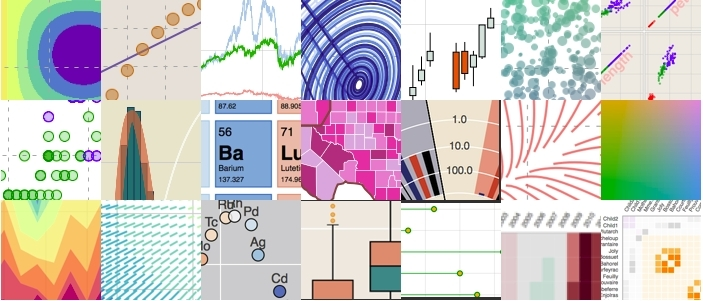
\includegraphics[width=.8\textwidth]{Pictures/bokehGallery.jpg}
\end{figure}
\begin{itemize}
\item Python plotting library (similar to matplotlib)
\item uses the webbrowser for displaying graphics
\item uses \texttt{D3.js}
\item open source
\item visit \url{http://bokeh.pydata.org}
\end{itemize}
\end{frame}

\begin{frame}[fragile]
\frametitle{\insertsubsection}
\begin{block}{static plotting in the browser}
\lstinputlisting[
commentstyle=\textbf,
language=Python,
basicstyle=\footnotesize]
{Examples/staticPlotting.py}
\end{block}
\end{frame}

\begin{frame}
\frametitle{\insertsubsection}
\begin{block}{Server example: An interactive function plotting tool}
\begin{itemize}
\item Start with \texttt{bokeh serve functionPlotter.py}
\item Visit \url{http://localhost:5006/functionPlotter}
\pause
\item only 60 LoC!
\item uses \texttt{numpy} and \texttt{scipy}
\end{itemize}
\end{block}
\end{frame}

\begin{frame}
\lstinputlisting[
commentstyle=\textbf,
language=Python,
basicstyle=\footnotesize]
{Examples/functionPlotterShort.py}
\end{frame}

\subsection{Example: Phase Plane Pictures}
\begin{frame}
\frametitle{\insertsubsection}
\begin{figure}
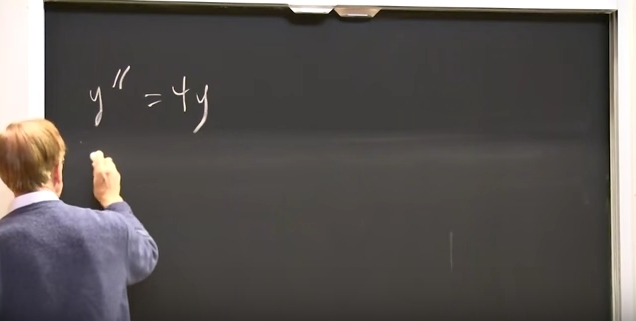
\includegraphics[width=.7\textwidth]{Pictures/Strang1.jpg}
\end{figure}
\pause
\begin{block}{2D ODE system}
\begin{align*}
y'' = u(x,y) & = 4y \\
y' = v(x,y) & = x
\end{align*}
Visualization on \url{http://localhost:5006/odesystem_app}
\end{block}
\end{frame}

\subsection{What do we get?}
\begin{frame}
\frametitle{\insertsubsection}
\begin{center}
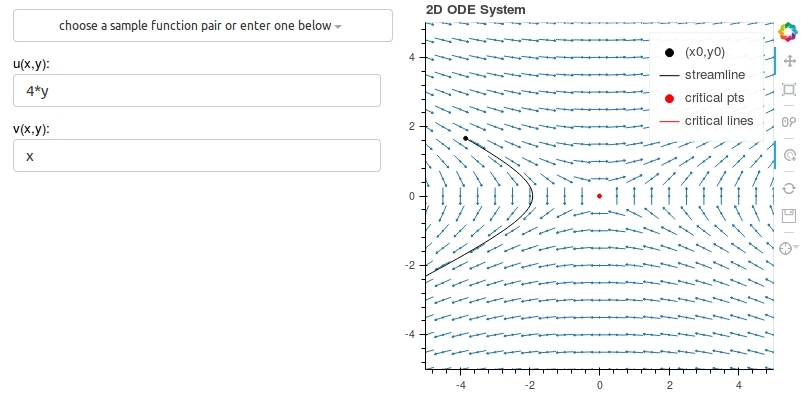
\includegraphics[height=.5\textheight]{Pictures/PhasePortraitPlot.jpg}
\end{center}
\begin{block}{Our goal}
\begin{itemize}
\citem Visualization of math content
\citem Easy-to-use, flexible tool
\citem For use at home and in lectures
\end{itemize}
\end{block}

\end{frame}

\begin{frame}
\frametitle{\insertsubsection}
\begin{block}{User Constraints}
\begin{itemize}
\citem No programming experience required
\citem No special tools required
\end{itemize}
\end{block}

\begin{block}{Development Constraints}
\begin{itemize}
\citem Easy to implement and understand
\citem Support for scientific applications
\end{itemize}
\end{block}

\begin{block}{BUT}
\begin{itemize}
\item we need a server
\item the user needs an internet connection
\item we have to transfer data
\item sometimes slow
\end{itemize}
\end{block}
\end{frame}

\section{Mini Pro \& Con}
\begin{frame}
\frametitle{\insertsection}
\Large{Go to lectures or use fancy tools?}
\pause
\begin{columns}
\begin{column}[t]{.45\textwidth}
\begin{block}{Lecture}
\begin{itemize}
\citem expert knowledge
\citem ask questions
\citem interpretation of results
\xitem sit \& relax
\xitem asking questions...
\end{itemize}
\end{block}
\end{column}
\begin{column}[t]{.45\textwidth}
\begin{block}{Fancy tools}
\begin{itemize}
\citem individual use
\citem check results
\citem explore algorithms
\xitem just pictures
\xitem no feedback
\xitem costly
\end{itemize}
\end{block}
\end{column}
\end{columns}
\end{frame}

\begin{frame}
\begin{columns}
\begin{column}{.5\textwidth}
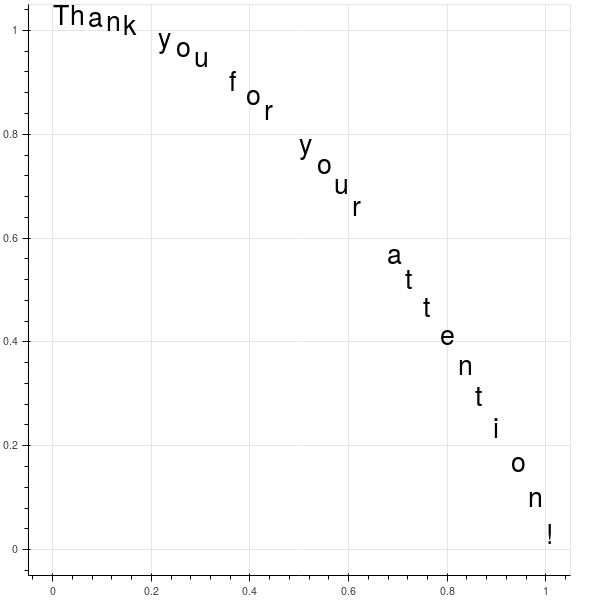
\includegraphics[width=\textwidth]{Pictures/thanks.png}
\end{column}
\begin{column}{.5\textwidth}
\lstinputlisting[
commentstyle=\textbf,
language=Python,
basicstyle=\tiny]{Examples/thanks.py}
\end{column}
\end{columns}

\end{frame}

\end{document}